\documentclass[12pt,addpoints,answers]{exam}
\usepackage{mystyle}
\usepackage[margin=0.4cm, landscape, b3paper]{geometry}

\begin{document}
\bracketedpoints
\pagestyle{headandfoot}
\mylogo
\begin{questions}
\question What is more likely? Provide quantitative support.
\begin{parts}
\part Obtaining at least one 6 in 4 rolls of a single die.
\part Obtaining at least one 12 in 24 rolls of a pair of dice.
\end{parts}
\question Mr.~Brown needs to take $1$ tablet of type $A$ and $1$ tablet of type $B$ together on a regular basis. One tablet of type $A$ corresponds to a $1$ mg dosage, and so does $1$ tablet of type $B.$ He keeps these two types of tablets in two separately labeled bottles as they cannot be differentiated easily. One day, on a busnesis trip, Mr.~Brown brought $10$ tablets of type $A$ and $10$ tablets of type $B.$. Unfortunately, he drops the bottles and breaks them. He does not have the time to go to a pharmacy to buy a new set of tablets but he needs to take his required dosage of both tablets $A$ and $B.$ The safe dosage that he needs for both tablets $A$ and $B$ is given by $$0.9\,\text{mg}\leq\text{safe dosage}\leq1.1\,\text{mg}.$$ Taking either an excess or a shortage of the required intake will result in serious health issues.
\begin{parts}
\part Suppose that after investigating the broken bottles, Mr.~Brown finds $2$ tablets that are still intact in the bottle for tablet $A.$ The other $18$ tablets are found to be mixed in a pile. Is it better for him to take one known tablet from the bottle and one from the pile, or take two tablets from the pile? Answer this by calculating the respective probabilities that he will not have any serious health issues for both options. 
\part Suppose that after investigating the broken bottles, Mr.~Brown finds that the tablets are all mixed up. What is the probability that he will not have any serious health issues if he randomly picks $2$ tablets?
\part In the previous part, Mr.~Brown randomly picked $2$ tablets. Instead of doing that, suppose now he decides to break each tablet in the pile into $10$ smaller pieces having exactly the same size, and then randomly pick $20$ pieces. What is the probability that he will not have any serious health issues?   
\end{parts}

\question Suppose we assume that 5\% of people in a specific population are drug users. A test is 95\% accurate; this means, that if the person is a drug user, the test result is positive 95\% of the time (\emph{true positive rate}) and if the person is not a drug user, the test result is negative 95\% of the time (\emph{true negative rate}). A random person tests positive. Is the individual highly likely to be a drug user?
\question Data was collected from the residents of a town and displayed as follows:
\begin{center}
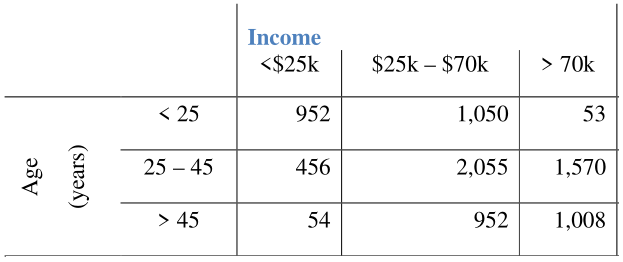
\includegraphics[keepaspectratio, scale = 0.6]{table.png}
\end{center}
Answer the following:
\begin{parts}
\part What fraction of people are less than 25 years old?
\part What is the probability that a randomly chosen person is more than 25 years old?
\part What fraction of people earn less than \$70,000?
\part What is the probability that a randomly chosen person is less than 25 years old and earns more than \$70,000?
\part What fraction of people among those who earn less than \$25,000 are between 25-45 years old?
\part If the next random person you see happens to be more than 45 years old, what is the probability that the person earns less than \$70,000?
\end{parts}
\question  You have tracked the performance of the local meteorologist and complied the following data:
\begin{center}
P(forecast rain, and actual rain) = 0.4, P(forecast rain, and no rain) = 0.2,\\
P(forecast no rain, and actual rain) = 0.15, P(forecast no rain, and no rain) = 0.25.
\end{center}
\begin{parts}
\part How often does she forecast rain?
\part How often does she make a mistake?
\part Given that she just forecast rain, what is the chance that it will actually rain?
\part Given that it rains today, what is the probability that she forecast rain in last
night's broadcast? 
\end{parts}
\question Consider a hash table with 5 buckets, where the probability of a string getting hashed to bucket $i$ is given by $p_i$ (where $\sum_{i=1}^5p_i=1.$) Now, 6 strings are hashed into the hash table.
\begin{parts}
\part Determine the probability that each of the first 4 buckets has at least 1 string hashed to each of them. Explicitly expand your answer in terms of $p_i,$ so that it does not include
any summations.
\part Assuming $p_1 = 0.1, p_2 = 0.25, p_3 = 0.3, p_4 = 0.25, p_5 = 0.1,$ simulate the problem using an R code and compare the computational answer with the theoretical answer derived above. Show your code snippet as part of your write up.
\end{parts}
\end{questions}
\label{totalpag}
\end{document}


 